\subsection{Fundamentals of astro-interferometry}
All the development of astro-interferometry is essentially based on one fundamental theorem : the Van Cittert-Zernike theorem. This theorem links the spatial coherence of a far source to its angular brightness distribution. In this section will be explained the limitation of one individual telescope in term of resolution and then introduce the advantages of interferometry. This section is based on \cite{Glindemann} and lectures given by J.P. Berger at Grenoble-INP Phelma. In order to fully understand the concepts lets first introduce the Mutual coherence function.

	\subsubsection{Mutual coherence function}
Lets consider the light field by its optical disturbance function $u(\vec{r},t)$ at position $\vec{r}$ and time $t$. The optical disturbance is proportional to the electrical and magnetic field of the light.
Lets suppose a far, coherent source illuminating two thin holes situated at position $\vec{r_1}$ and $\vec{r_2}$ (like the young experiment) and forming fringe pattern on a screen. At a point P ant time t of the screen the intensity of the light can be expressed by :
$I(P) = \left< u(P,t)u^*(P,t) \right>$ which can be rewritten if we consider the holes thin enough that the field is constant on their respective surface :
$$
I(P) = \left< \left| u(\vec{r_1},t-\tau_1) \right|^2 \right> + \left< \left| u(\vec{r_2},t-\tau_2) \right|^2 \right> +2\mathcal{R}\left( \left< \left| u(\vec{r_1},t-\tau_1)u^*(\vec{r_2},t-\tau_2) \right| \right> \right)
$$
where $\tau_1$ and $\tau_2$ refers to the travel time of the wave from the pin hole to the point P. The last term of this equation is a term of coherence representing the spatial and spectra properties of the source. From this equation we can generalise the measurement of the coherence of a source by introducing the mutual coherence function (MCF) :
\begin{equation}
\Gamma(\vec{r_1},\vec{r_2}, \tau) = \left< u(\vec{r_1},t+\tau)u^*(\vec{r_2},t)\right> = \lim\limits_{T\rightarrow +\infty}\int_{-T}^T u(\vec{r_1},t+\tau)u^*(\vec{r_2},t)dt
\end{equation} 

In the case of astrointerferometry the two pinholes refers to the telescopes and the source to the observed object. The distance between both telescopes is called the baseline vector $\vec{B}=\vec{r_1}-\vec{r_2}$. 

	\subsubsection{Van Cittert-Zernike theorem}
Now that the MCF has been defined the most fundamental theorem of modern optic can be introduced. We will consider the Van Cittert-Zernike theorem in an adapted to astronomy form. We will consider a surface emitting light. Under the following assumption :
\begin{itemize}
\item[-]The source is incoherent ($\Gamma(P_1,P_2,\tau) = 0 \quad P_1 \neq P_2$ for all $\tau$)
\item[-]The source is small compared to the distance of observation (Fresnel approximation)
\item[-]The source spectral bandwidth is much smaller than its average frequency (quasi-monochromatic approximation).
\end{itemize}

\begin{figure}[htbp!]
\centering
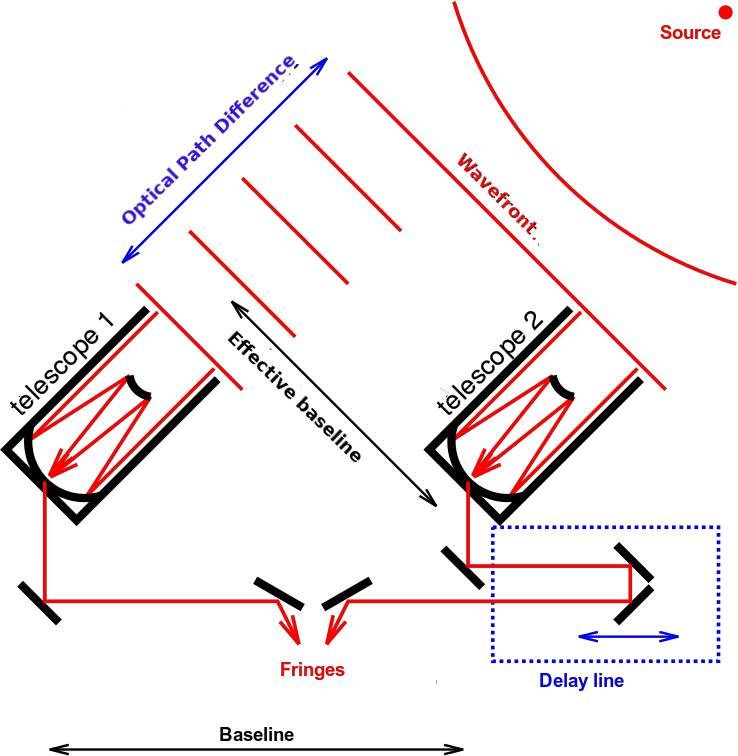
\includegraphics[scale=.3]{../images/scheme.png}
\caption{Scheme of the principle of stellar interferometry. }
\end{figure}

Under those assumptions the Van Cittert-Zernike theorem states that :
$$
\mu(\vec{B}) = \frac{\Gamma(\vec{B},0)}{\sqrt(\Gamma{\vec{r_1},\vec{r_1},0)\Gamma(\vec{r_2},\vec{r_2},0)}} = \frac{\int I_b(\vec{\alpha}) e^{-ik\vec{B} \cdot \vec{\alpha}}}{d\vec{\alpha}}
$$

where alpha is the angle between the line of sight and a point on the observed source and $\mu$ the normalised MCF at $\tau=0$, called the visibility function. $I_b(\vec{\alpha})$ is the angular brightness distribution of the source. 

	\subsubsection{Spatial resolution}